%
% This file is part of Calicut University Question Paper Collection.
%
% Copyright (c) 2012-2015 Mohammed Sadik P. K. <sadiq (at) sadiqpk (d0t) org>.
% License: GNU GPLv3 or later
%
% Calicut University Question Paper Collection is free software: you can
% redistribute it and/or modify
% it under the terms of the GNU General Public License as published by
% the Free Software Foundation, either version 3 of the License, or
% (at your option) any later version.
% 
% Calicut University Question Paper Collection is distributed in the hope
% that it will be useful,
% but WITHOUT ANY WARRANTY; without even the implied warranty of
% MERCHANTABILITY or FITNESS FOR A PARTICULAR PURPOSE.  See the
% GNU General Public License for more details.
% 
% You should have received a copy of the GNU General Public License
% along with Calicut University Question Paper Collection.
% If not, see <http://www.gnu.org/licenses/>.
% 
%

\def \subj{AI 09 503---CONTROL ENGINEERING}

\mainhead{50628}{2}
\semfive{NOVEMBER 2013}
\sub{\subj}

\maxtime
\partA

\iitem Define closed loop system.
\item Write the torque balance equation of an ideal rotational mass
  element.
\item What is steady state and transient response.
\item Define pole and zero.
\item Define controllability and observability.

\markA
\partB

\item Explain the rule
\iitem for eliminating negative feedback loop
\item for moving the summing point ahead of a block.
\ene
\item State and explain the principle of superposition and homogeneity.
\item Explain first order and second order systems and their significance.
\item Explain lag and lead compensation.
\item State and explain Cayley Hamilton theorem.
\item A discrete type system is described by the difference equation,\\
  $y(k + 2) + 3y(k + 1) + 5y (k) = u(k)$. Determine the transfer function
  of the system.

\markB

\newpage \again

\partC

\item \iitem \iitem State and explain Mason's gain formula.
\item Explain basic properties of signal flow graph.
\ene
\Or
\item Write the analogous electrical elements in
  (i) force-voltage (ii) force-current and (iii) torque-voltage
  analogy for the elements of mechanical systems.
\ene

\item \iitem Sketch the root locus for the unity feedback system whose
  open loop transfer function is
  \[ G(s) = \dfrac{K(s^2 + 6s + 25)}{s (s + 1) (s + 2)}\]
\Or
\item Discuss in detail about Routh Hurwitz stability criterion.
\ene

\item \iitem Sketch the bode plot for the following transfer function
  and determine phase margin and gain margin.
  \[ G(s) = \dfrac{75 (1 + 0.2s)}{s (s^2 + 16s + 100)}\]
\Or
\item The open loop transfer function of a system is given by
  \[ G(s) = \dfrac{K}{s (1 + 0.5s) ( 1 + 0.2s)}\]
  Using bode plot find the value of $k$ so that (i) the gain margin of
  the system is 6 dB and (ii) the phase margin of the system is 25$^\circ$.
\ene

\item \iitem What is state transition matrix? Explain its properties. Obtain
  the state model of the system whose transfer function is
  $\dfrac {1}{s^2 + 3s + 2}$.
\Or
\item A discrete-type system has the transfer function
  \[ \dfrac{Y(Z)}{U(Z)} = \dfrac{(4Z^3 - 12Z^2 + 13Z - 7)}{(Z-1)^2(Z-2)} \]
  determine the state model of the system (i) Phase variable form and \\(ii)
  Jordan Canonical form
\ene

\markC
\ene

\newpage

\mainhead{30970}{2}
\semfive{NOVEMBER 2012}
\sub{\subj}

\maxtime
\partA

\iitem State the difference between open loop and closed loop control systems.
\item State Mason's Gain Formula.
\item State the difference between absolute stability and relative stability.
\item Define Gain Margin and Phase Margin.
\item Define Controllability and Observability.

\markA
\partB

\item What is a transfer function? Derive the transfer function of the network shown
  in Fig. 1.

\begin{center}
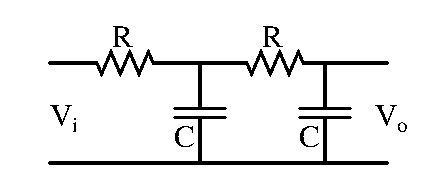
\includegraphics{src/s5/ai/09_503/fig001}
\end{center}
\item Calculate the time response of the following system if the input r(t) is an unit
  impulse $ \dfrac{C(s)}{R(s)} = \dfrac{2}{s+3}$.
\item Write the Hurwitz determinant for the system given by the characteristic equation

  $4s^3 + 2s^2 + 5s + 7 = 0$.
\item With neat sketch explain the underdamped and overdamped second order systems.
\item Briefly explain the minimum phase and non-minimum phase systems.

\newpage \again

\item With a suitable example, explain the canonical form representation.

\markB
\partC

\item \iitem With a suitable example, Explain the transfer function of a simple electrical
  and electromechanical systems.
\Or
\item Explain the rules for block diagram reduction.
\ene

\item \iitem Discuss in detail about the various standard test signals.
\Or
\item Sketch the root locus plot of a unity feedback system with an open loop transfer
  function
  \[ G(s) = \frac{K}{s (s + 2) (s + 4)} \]

  Determine the value of K so that the dominant pair of complex poles of the system has a damping
  ratio of 0.5.
\ene

\item \iitem The open loop transfer function of a unity feedback control system is 
  \[ G (s) = \frac{K}{s (1 + 0.1s) (1 + s)} \]
  
  Draw the Bode diagram and analyze the stability of the system for K = 10.
\Or
\item Discuss in detail about Nyquist stability criterion.
\ene

\item \iitem Explain (i) State variable (ii) State vector (iii) State space (iv) State diagram.
\Or
\item Explain the computation of state transition matrix using (i) Laplace transform and 
  (ii) Cayley Hamilton theorem.
\ene

\markC
\ene

\newpage

\mainhead{20919}{3}
\semfive{OCTOBER 2011}
\sub{\subj}
\maxtime
\partA

\iitem Define transfer function.
\item What is the significance of impulse response?
\item What is the relation between gain margin and steady 
  state error?
\item State any two advantages of State representation.
\item Define controllability and observability.

\markA
\partB

\item write a note on open loop and closed loop systems.
\item A servomechanism has inertia $17 \times 10^{-6} kgm^2$, viscous friction
  $ 680 \times 10^{-6}$ Nm/rad/sec, and controller constant 0.0068 Nm/radians error.
  Find an expression for the error angle as a function of time when the input begins
  to rotate at 3 rev/min. Also find the natural frequency of the system.
\item Briefly explain about any two standard test signals.
\item What are absolute and relative stability?
\item What are M-N circles?
\item Obtain a state space representation of the system governed by the
  differential equation.
  \[ \dfrac{\ud^2y}{\ud t^2} + 3 \dfrac{\ud y}{\ud t} + 2y = 2\dfrac{\ud u}{\ud t} + 6u \]

\newpage \again

\markB
\partC

\item \iitem What are the two types of analogies between electrical and mechanical systems?
  Explain them in detail.
\item State Mason's Gain Formula. Explain how the transfer function is
  determined using Mason's Gain formula.
\ene
\Or
\item A DC motor drive a pointer which is spring loaded to return to the
  reference position. If K$_\text{b}$ = back \emph{emf} constant, K$_\text{t}$ 
  = torque constant, K$_\text{s}$ Spring constant and J moment of inertia, find
  the transfer function

\item Discuss in detail about time response of a 
  (a) First order system
  (b) Second order system
\Or
\item Examine the stability by Routh's Criterion of the system whose characteristic equation is
  $s^5 + s^4 + 2s^3 + 2s^2 + 3s + 15 = 0$.

\item A unity feedback system has G(s)$ = \frac{k}{s(1 + \text{T}_s)}$. When subjected
  to using step input, it shows 30\% peak overshoot while it shows resonant frequency
  of 10 rad/sec in frequency domain. Calculate K and T. Also calculate
  (a) Gain cross over frequency 
  (b) Phase cross over frequency and\\
  (c) resonant peak.
\Or
\item Draw the Bode plot for a unity feedback system with

\[ G(s) = \dfrac{k(s + 0.3)}{(s + 4)(s^2 + 30s + 20)}\]

where k = 2000. Determine gain margin, Phase margin. Comment on stability.
Determine the value of k to obtain phase margin of 30$^\circ$.

\item Consider a system given by the following equation
\[ \dfrac{\ud^3y}{\ud t^3} + 9{\ud^2y}{\ud t^2} + 26\dfrac{\ud y}{\ud t} + 24y = 6u\]

Find the canonical form of the state space equations by using partial fraction method.
\Or
\item Obtain canonical state model of the system whose transfer function is
\[ \text{T}(s) = s + \dfrac{5}{(s + 1)(s + 2)(s + 3)} \]

\markC
\ene
